\documentclass{beamer}
% \usepackage{pgfpages}
% \pgfpagesuselayout{4 on 1}[a4paper,landscape,border shrink=5mm]
\usepackage{tikz}
\usetikzlibrary{shapes, backgrounds, arrows, positioning}
%\usepackage{pgfplots}
\usepackage{listings}
\usepackage[utf8,latin1]{inputenc}
\usepackage[natbibapa]{apacite}
\makeatletter \def\newblock{\beamer@newblock} \makeatother  

\beamertemplatenavigationsymbolsempty
\setbeamertemplate{itemize items}[circle]
\setbeamertemplate{section in toc}[circle]
\mode<beamer>{\setbeamercolor{math text displayed}{fg=iwmgrau}}
\setbeamercolor{block body}{bg=iwmorange!50!white}
\setbeamercolor{block title}{fg=white, bg=iwmorange}

\definecolor{iwmorange}{RGB}{255,105,0}
\definecolor{iwmgrau}{RGB}{67,79,79}
\setbeamercolor{title}{fg=iwmorange}
\setbeamercolor{frametitle}{fg=iwmorange}
\setbeamercolor{structure}{fg=iwmorange}
\setbeamercolor{normal text}{fg=iwmgrau}
\setbeamercolor{author}{fg=iwmgrau}
\setbeamercolor{date}{fg=iwmgrau}

\title{Repeated measures}
\author{Nora Umbach%\footnote{These slides are a modified version of slides created by \url{https://osf.io/ /}. }
}
%\institute{\includegraphics[scale=.15]{figures/ut_logo}}
\date{June 14, 2021}
%\date{Last modified: \today}

\newcommand{\vect}[1]{\mathbf{#1}}
\newcommand{\mat}[1]{\mathbf{#1}}
\newcommand{\gvect}[1]{\boldsymbol{#1}}
\newcommand{\gmat}[1]{\boldsymbol{#1}}

\lstset{language=R,%
  literate={Ü}{{\"U}}1
           {ü}{{\"u}}1,
  %backgroundcolor=\color{iwmgrau!80!white},
  basicstyle=\ttfamily\color{iwmorange},
  frame=single,
  commentstyle=\slshape\color{black},
  keywordstyle=\bfseries\color{white},
  identifierstyle=\color{white},
  stringstyle=\color{green!85!black},
  numbers=none,%left,numberstyle=\tiny,
  basewidth={.5em, .4em},
  showstringspaces=false,
  emphstyle=\color{red!50!white}}

\lstdefinestyle{plain}{language=R,
  frame=none,
  basicstyle=\ttfamily\color{iwmorange},
  commentstyle=\slshape\color{iwmgrau},
  keywordstyle=\bfseries\color{iwmgrau},
  identifierstyle=\color{iwmgrau},
  stringstyle=\color{iwmgrau},
  numbers=none,
  basewidth={.5em, .4em},
  showstringspaces=false}

\pgfmathdeclarefunction{gauss}{2}{%
  \pgfmathparse{1/(#2*sqrt(2*pi))*exp(-((x-#1)^2)/(2*#2^2))}%
}

\AtBeginSection[]{
  \frame{
    \tableofcontents[sectionstyle=show/hide, subsectionstyle=show/show/hide]}}

\setbeamertemplate{headline}{
 \begin{beamercolorbox}{section in head}
   \vskip5pt\insertsectionnavigationhorizontal{\paperwidth}{}{}\vskip2pt
 \end{beamercolorbox}
}

\setbeamertemplate{footline}{\vskip-2pt\hfill\insertframenumber$\;$\vskip2pt}

\begin{document}

\begin{frame}{}
\thispagestyle{empty}
\titlepage
\end{frame}

% \begin{frame}{Outline}
% \tableofcontents
% \end{frame}


\begin{frame}{Example: Depression and Imipramin}
  \begin{itemize}
    \item \citet{ReisbyGram77} studied the effect of Imipramin on 66
      inpatients treated for depression
    \item Depression was measured with the Hamilton depression rating scale
      (HDRS)
    \item Additionally, the concentration of Imipramin and its metabolite
      Desipramin was measured in their blood plasma
    \item Patients were classified into endogenous and non-endogenous
      depressed
    \item Depression was measured weekly for 6 time points; the effect of
      the antidepressant was observed starting at week 2 for four weeks
  \end{itemize}
\end{frame}

\begin{frame}{Example: Depression and Imipramin}
  {\citep{ReisbyGram77}}
\begin{center}
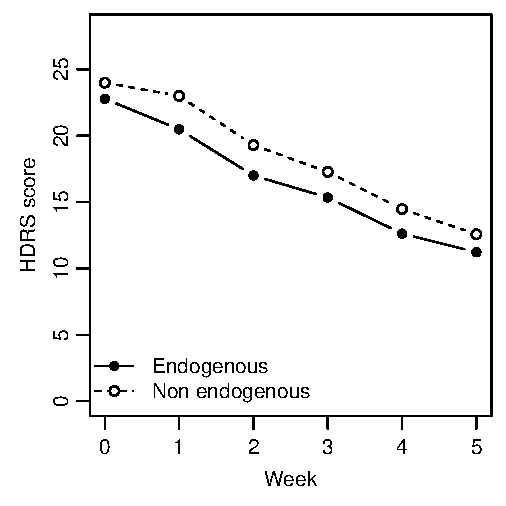
\includegraphics[scale=.8]{figures/hdrs-means}
\end{center}
\end{frame}

\begin{frame}{Excursion: Repeated measures ANOVA}
  {Model with one repeated measurement factor}
  \begin{itemize}
    \item When subjects are observed for more than two time points, we can
      model these data using a repeated measures ANOVA; then, the repeated
      measures factor is time
    \item Data layout
\[ \begin{array}{c|cccccc}
              & \multicolumn{6}{c}{\text{Time point}} \\
\text{Subject} & 1 & 2 & \cdots & j & \cdots & n \\ \hline
1      & y_{11} & y_{12} & \cdots & y_{1j} & \cdots & y_{1n} \\
2      & y_{21} & y_{22} & \cdots & y_{2j} & \cdots & y_{2n} \\
\vdots & \vdots &        &        &        &        & \vdots \\
i      & y_{i1} & y_{i2} & \cdots & y_{ij} & \cdots & y_{in} \\
\vdots & \vdots &        &        &        &        & \vdots \\
N      & y_{N1} & y_{N2} & \cdots & y_{Nj} & \cdots & y_{Nn} \\
\end{array} \]
  \end{itemize}
\end{frame}


\begin{frame}{Excursion: Repeated measures ANOVA}
  {Statistical model}
  \begin{itemize}
    \item When we observe $i = 1, \ldots, N$ subjects for $j = 1, \ldots,
      n$ time points, we get
\[
  y_{ij} = \mu_0 + \tau_j + \upsilon_i + \varepsilon_{ij}
\]
with $\mu_0 :=$ grand mean, $\upsilon_i := $ effect of subject $i$ constant over
  time, $\tau_j :=$ effect of time point $j$ equal
  for all subjects, $\varepsilon_{ij} :=$ error term for subject $i$ at time point
  $j$

\item It is assumed that $\upsilon_i \sim N(0, \sigma^2_\upsilon)$ i.i.d.
  with $\sigma^2_\upsilon$ being the variance between subjects,
      $\varepsilon_{ij} \sim N(0, \sigma^2)$ i.i.d. with $\sigma^2$ being
      the variance within subjects
    \item Additionally, $\upsilon_i$ and $\varepsilon_{ij}$ are independent
  \end{itemize}
\end{frame}

\begin{frame}{Excursion: Repeated measures ANOVA}
  {Statistical model}
  \[
  y_{ij} = \mu_0 + \tau_j + \upsilon_i + \varepsilon_{ij}
  \]

  \begin{tabular}{ccccc}
    \hline
    response & grand mean & time effect & subject effect  & residual \\
    \hline
    $y_{11}$ & $\mu_0$ & $\tau_1$  & $\upsilon_{1}$ & $\varepsilon_{11}$ \\
    $y_{12}$ & $\mu_0$ & $\tau_2$  & $\upsilon_{1}$ & $\varepsilon_{12}$ \\
    $y_{13}$ & $\mu_0$ & $\tau_3$  & $\upsilon_{1}$ & $\varepsilon_{13}$ \\
    \vdots & \vdots & \vdots   &  \vdots & \vdots \\
    $y_{21}$ & $\mu_0$ & $\tau_1$  & $\upsilon_{2}$ & $\varepsilon_{21}$ \\
    $y_{22}$ & $\mu_0$ & $\tau_2$  & $\upsilon_{2}$ & $\varepsilon_{22}$ \\
    $y_{23}$ & $\mu_0$ & $\tau_3$  & $\upsilon_{2}$ & $\varepsilon_{23}$ \\
    \vdots & \vdots & \vdots   &  \vdots & \vdots \\
    $y_{Nn}$ & $\mu_0$ & $\tau_n$  & $\upsilon_{N}$ & $\varepsilon_{Nn}$ \\
    \hline\\[-2ex]
    \only<2>{$\sigma_{\upsilon}^2 + \sigma_{\varepsilon}^2$ & & &
    $\sigma_{\upsilon}^2$ & $\sigma_{\varepsilon}^2$} \\
  \end{tabular}
\end{frame}

\begin{frame}{Excursion: Repeated measures ANOVA}
  {Model properties}
  \begin{itemize}
    \item For the model, we have
\begin{align*}
  E(y_{ij})   &= \mu_0 + \tau_j \\
  Var(y_{ij}) &= Var(\mu_0 + \upsilon_i + \tau_j + \varepsilon_{ij})
               = \sigma^2_\upsilon + \sigma^2 \\
  Cov(y_{ij}, y_{i'j}) &= 0 \text{ for subjects } i \neq i' \\
  Cov(y_{ij}, y_{ij'}) &= \sigma^2_\upsilon \text{ for observations }
                          j \neq j'
\end{align*}
      \vspace{-.6cm}
\item The correlation between observations and subjects is
\[
  Corr(y_{ij}, y_{ij'}) = \frac{\sigma^2_\upsilon}{\sigma^2_\upsilon +
    \sigma^2}
\]
intraclass correlation (ICC)
  \end{itemize}
\end{frame}

\begin{frame}{Excursion: Repeated measures ANOVA}
{Compound Symmetry}
  \begin{itemize}
    \item Thus, we get for the covariance matrix of the observations for
      one subject the so-called compound symmetry structure
\[
  \gvect{\Sigma}_{\vect{y}_i} = \sigma^2_\upsilon \vect{1} \vect{1}'
    + \sigma^2 \mat{I}
  = 
  \begin{pmatrix}
    \sigma^2_\upsilon + \sigma^2 & \sigma^2_\upsilon & \sigma^2_\upsilon &
      \cdots & \sigma^2_\upsilon \\
    \sigma^2_\upsilon & \sigma^2_\upsilon  + \sigma^2 & \sigma^2_\upsilon &
      \cdots & \sigma^2_\upsilon \\
    \vdots & & \ddots & & \vdots \\
    \sigma^2_\upsilon & \sigma^2_\upsilon  & \sigma^2_\upsilon &
      \cdots & \sigma^2_\upsilon + \sigma^2 \\
  \end{pmatrix}
\]
% \item The covariance matrix for all observations is consequently block diagonal
% \[
%   Cov(\vect{y}) =
%   \begin{pmatrix}
%   \gvect{\Sigma}_{\vect{y}_1} & 0 & 0 & \cdots & 0 \\
%   0  & \gvect{\Sigma}_{\vect{y}_2} & 0 & \cdots & 0 \\
%   \vdots &  & \ddots &  & \vdots \\
%   0 & 0 & 0 & \cdots & \gvect{\Sigma}_{\vect{y}_N} \\
%   \end{pmatrix}
% \]
% and, therefore, $Cov(\vect{y}) = \sigma^2 \mat{I}$ does not apply as in the
%   regular linear model
  \end{itemize}
\end{frame}


\begin{frame}{Excursion: Repeated measures ANOVA}
{Compound Symmetry}
  \begin{itemize}
    \item The assumption of a compound symmetry structure for the
      covariance matrix for longitudinal data is usually unrealistic
    \item In general, successive observations are more strongly correlated
      than observations being farther apart (covariance is not constant);
      variance increases with time, e.\,g., when some subjects are more
      responsive to a certain treatment than others
    \item In order to test for compound symmetry or the weaker sphericity,
      tests have been proposed (e.\,g., Mauchly test) but these tests do
      not possess good statistical qualities
  \end{itemize}
\end{frame}



\begin{frame}{Depression and Imipramin: Descriptive statistics}
  {\citep{ReisbyGram77}}
\begin{columns}
\begin{column}{12cm}
HDRS score
\begin{center}
\begin{tabular}{rrrrrrr}
  \hline
  $t$ & Week 0 & Week 1 & Week 2 & Week 3 & Week 4 & Week 5 \\ 
  \hline
  $M$  & 23.44 & 21.84 & 18.31 & 16.42 & 13.62 & 11.95 \\ 
  $SD$ &  4.53 & 4.70  & 5.49  & 6.42  & 6.97  & 7.22 \\ 
  $n$  & 61    & 63    & 65    & 65    & 63    & 58    \\ 
  \hline
\end{tabular}
\end{center}
Empirical correlation matrix of HDRS score
\begin{center}
\begin{tabular}{rrrrrrr}
  \hline
   & W0 & W1 & W2 & W3 & W4 & W5 \\ 
  \hline
  Week 0 &   1 & .49 & .41 & .33 & .23 & .18 \\ 
  Week 1 & .49 &   1 & .49 & .41 & .31 & .22 \\ 
  Week 2 & .41 & .49 &   1 & .74 & .67 & .46 \\ 
  Week 3 & .33 & .41 & .74 &   1 & .82 & .57 \\ 
  Week 4 & .23 & .31 & .67 & .82 &   1 & .65 \\ 
  Week 5 & .18 & .22 & .46 & .57 & .65 &   1 \\ 
  \hline
\end{tabular}
\end{center}
\end{column}
\end{columns}
\end{frame}

\begin{frame}{Depression and Imipramin: Descriptive statistics}
  {\citep{ReisbyGram77}}
\begin{center}
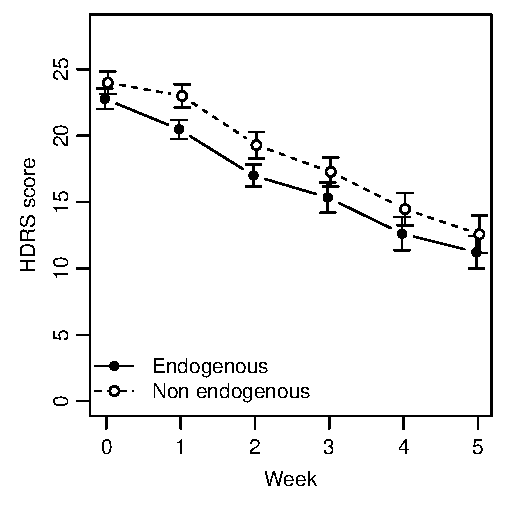
\includegraphics[scale=.8]{figures/hdrs-means-se}
\end{center}
\end{frame}

{\setbeamercolor{background canvas}{bg=iwmgrau!80!white}

\begin{frame}[fragile]{Depression and Imipramin}
  \begin{lstlisting}
dat      <- read.table("reisby.dat", header=TRUE)
dat$id   <- factor(dat$id)
dat$diag <- factor(dat$diag, 
                   levels=c("nonen", "endog"))
dat      <- na.omit(dat)     # drop missing values

# Descriptive statistics
aggregate(hamd ~ week, dat, mean)
aggregate(hamd ~ week, dat, sd)
aggregate(hamd ~ week, dat, length)

cor(reshape(dat[, c("hamd", "id", "week")], 
            direction="wide",
            timevar="week")[, 2:7],
    use="pairwise.complete.obs")
  \end{lstlisting}
\end{frame}

}

{\setbeamercolor{background canvas}{bg=iwmgrau!80!white}

\begin{frame}[fragile]{Fitting repeated-measures ANOVA}
  \begin{lstlisting}
# Week needs to be a factor when computing a ANOVA
dat$week2 <- factor(dat$week)
summary(aov(hamd ~ week2*diag + Error(id/week2), dat))
# --> ?? 

library(ez)   # "SPSS"-style
ezANOVA(data = dat, dv = hamd, wid = id,
        within = week2, between = diag, type = 3)

# Check data
ezDesign(data = dat, x = week, y = id, col = diag)
  \end{lstlisting}
\end{frame}

\begin{frame}[fragile]{Fitting repeated-measures ANOVA}
  \begin{lstlisting}
# Remove IDs with missing observations
ids <- names(which( addmargins(
  xtabs( ~ week + diag + id, dat) )
  ["Sum", "Sum",] == 6))
dat_val <- dat[dat$id %in% ids, ]

# Fit ANOVAs again
aov1 <- aov(hamd ~ week2*diag + Error(id/week2),
            dat_val)
summary(aov1)

ez1 <- ezANOVA(data = dat_val, dv = hamd, wid = id,
               within = week2, between = diag,
               type = 3)
ez1$ANOVA
  \end{lstlisting}
\end{frame}

\begin{frame}[fragile]{Fitting repeated-measures ANOVA}
  \begin{lstlisting}
# How close can we get with a mixed-effects model?
library(lme4)

lme1 <- lmer(hamd ~ week2*diag + (1 | id),
            dat_val)
anova(lme1)

# Calculate mean sum of squares for id by hand
sp <- attr(VarCorr(lme1)$id, "stddev")
se <- attr(VarCorr(lme1), "sc")
se^2 + 6*sp^2
  \end{lstlisting}
\end{frame}

\begin{frame}[fragile]{Fitting mixed-effects model}
  \begin{lstlisting}
# And this works on the complete data set
lme2 <- lmer(hamd ~ week2*diag + (1 | id), dat)
anova(lme2)

# Type I sum of squares
m0 <- lmer(hamd ~ 1 + (1 | id), dat, REML=FALSE)
m1 <- lmer(hamd ~ week2 + (1 | id), dat, REML=FALSE)
m2 <- lmer(hamd ~ week2 + diag + (1 | id), dat,
           REML=FALSE)
anova(m0, m1, m2, lme2)
  \end{lstlisting}
\end{frame}

}

\begin{frame}{Alternative model with a constant time term}
  \centering
  \vspace{-1cm}
  \[
  y_{ij} = \beta_0 + \beta_1 \cdot time + \upsilon_i + \varepsilon_{ij}
  \]
  with $\varepsilon_{ij} \sim N(0, \sigma_{\varepsilon}^2)$ i.i.d.\ and
  $\upsilon_{0i} \sim N(0, \sigma_{\upsilon})$ i.i.d.\\~\\

  \begin{tabular}{cccccc}
    \hline
    response & intercept & time effect & time & subject effect  & residual \\
    \hline
    $y_{11}$ & $\beta_0$ & $\beta_1$   & 0    & $\upsilon_{1}$ & $\varepsilon_{11}$ \\
    $y_{12}$ & $\beta_0$ & $\beta_1$   & 1    & $\upsilon_{1}$ & $\varepsilon_{12}$ \\
    $y_{13}$ & $\beta_0$ & $\beta_1$   & 2    & $\upsilon_{1}$ & $\varepsilon_{13}$ \\
    \vdots & \vdots & \vdots   & \vdots & \vdots & \vdots \\
    $y_{21}$ & $\beta_0$ & $\beta_1$   & 0    & $\upsilon_{2}$ & $\varepsilon_{21}$ \\
    $y_{22}$ & $\beta_0$ & $\beta_1$   & 1    & $\upsilon_{2}$ & $\varepsilon_{22}$ \\
    $y_{23}$ & $\beta_0$ & $\beta_1$   & 2    & $\upsilon_{2}$ & $\varepsilon_{23}$ \\
    \vdots & \vdots & \vdots   & \vdots & \vdots & \vdots \\
    $y_{Nn}$ & $\beta_0$ & $\beta_1$   & n    & $\upsilon_{N}$ & $\varepsilon_{Nn}$ \\
    \hline
  \end{tabular}
\end{frame}

\begin{frame}{Depression and Imipramin: Individual process}
  {\citep{ReisbyGram77}}
\begin{columns}
\begin{column}{12cm}
\vspace{-.45cm}
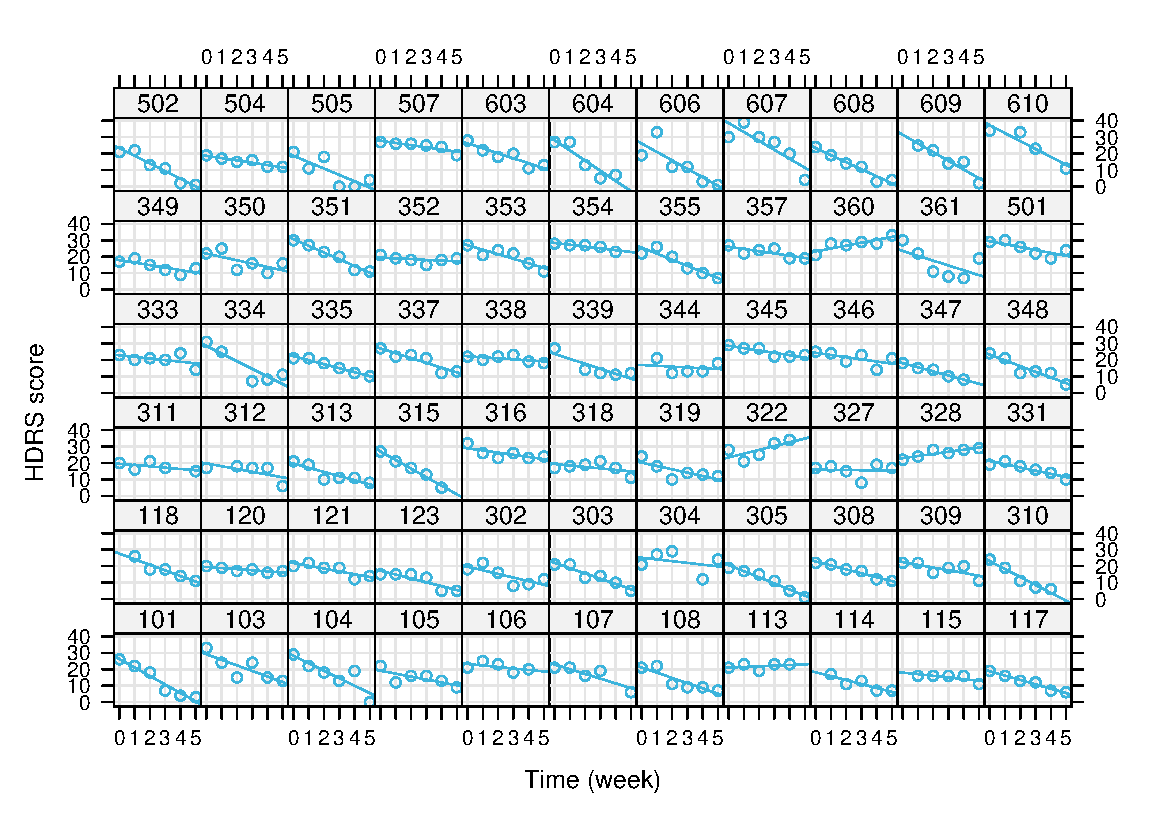
\includegraphics[width=11cm]{figures/hdrs-ind}
\end{column}
\end{columns}
\end{frame}

\begin{frame}[fragile]{Random intercept model}
\begin{align*}
\text{(Level 1)}  \quad y_{ij} &= b_{0i} + b_{1i}\,t_{ij} + \varepsilon_{ij}\\
\text{(Level 2)}  \quad b_{0i} &= \beta_0 + \upsilon_{0i}\\
                  \quad b_{1i} &= \beta_1\\
\text{(2) in (1)} \quad y_{ij} &= \beta_0 + \beta_1\,t_{ij} +
                                  \upsilon_{0i} + \varepsilon_{ij}
\end{align*}
with $\upsilon_{0i} \sim N(0, \sigma^2_{\upsilon})$ i.i.d.,
$\varepsilon_{ij} \sim N(0, \sigma^2)$ i.i.d., $\upsilon_{0i}$ and
$\varepsilon_{ij}$ i.i.d.\\[2ex]

Fitting the mixed-effects model in R
\begin{lstlisting}[style=plain]
lme1 <- lmer(hamd ~ week + (1 | id), dat, REML=FALSE)
\end{lstlisting}
\end{frame}

% \begin{frame}[fragile]{ML estimation of parameters}
% \begin{lstlisting}
% Linear mixed model fit by maximum likelihood  ['lmerMod']
% Formula: hamd ~ week + (1 | id)
%    Data: dat
%       AIC       BIC    logLik  deviance  df.resid 
%  2293.189  2308.896 -1142.594  2285.189       371 
% Random effects:
%  Groups   Name        Std.Dev.
%  id       (Intercept) 4.019   
%  Residual             4.363   
% Number of obs: 375, groups:  id, 66
% Fixed Effects:
% (Intercept)         week  
%      23.552       -2.376  
% \end{lstlisting}
% \end{frame}


\begin{frame}{Model predictions}
\begin{columns}
\begin{column}{6cm}
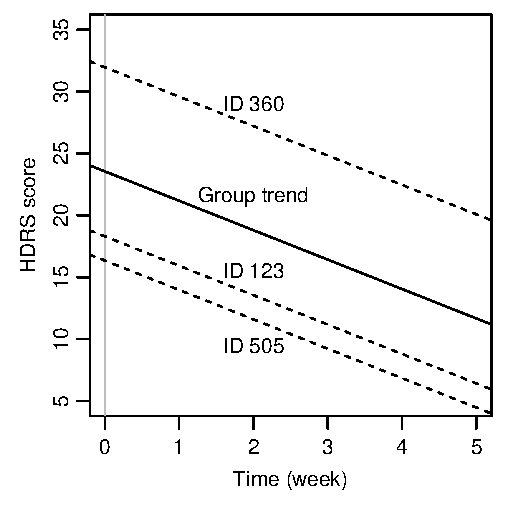
\includegraphics[width=6cm]{figures/hdrs-lme1}
\end{column}
%
\begin{column}{5cm}
  The estimated mean baseline HDRS score is $\hat{\beta}_0 = 23.55$\\[2ex]

  However, the estimated standard deviation between patients is
  $\hat{\sigma}_\upsilon = 4.02$.\\[2ex]

  The mean improvement per week is $\hat{\beta}_1 = -2.38$
\end{column}
\end{columns}
\end{frame}


\begin{frame}{Implied marginal covariance matrix}
For the three time points $t_{ij} = 0, 1, 2$, $\mat{Z}_i = \vect{1}'_{n_i}$
  and $\gmat{\Sigma}_\upsilon = \sigma^2_\upsilon$ we get
\begin{align*}
  Cov(\vect{y}_i) &=
    \mat{Z}_i \gmat{\Sigma}_\upsilon \mat{Z}'_i + \sigma^2 \mat{I}_{n_i} \\
  &= \sigma^2_\upsilon \vect{1}_{n_i} \vect{1}'_{n_i} +
     \sigma^2 \mat{I}_{n_i} \\
  &= 
  \begin{pmatrix}
    \sigma^2_\upsilon + \sigma^2 & \sigma^2_\upsilon & \sigma^2_\upsilon \\
    \sigma^2_\upsilon & \sigma^2_\upsilon + \sigma^2 & \sigma^2_\upsilon \\
    \sigma^2_\upsilon & \sigma^2_\upsilon & \sigma^2_\upsilon + \sigma^2
  \end{pmatrix}
\end{align*}
The random intercept model implies the compound symmetry structure
\end{frame}

\begin{frame}[fragile]{Random slope model}
\begin{align*}
\text{(Level 1)}  \quad y_{ij} &= b_{0i} + b_{1i}\,t_{ij} + \varepsilon_{ij}\\
\text{(Level 2)}  \quad b_{0i} &= \beta_0 + \upsilon_{0i}\\
                  \quad b_{1i} &= \beta_1 + \upsilon_{1i}\\
\text{(2) in (1)} \quad y_{ij} &= \beta_0 + \beta_1\,t_{ij} +
                   \upsilon_{0i} + \upsilon_{1i} \, t_{ij}+ \varepsilon_{ij}
\end{align*}
with
\begin{align*}
  \begin{pmatrix} \upsilon_{0i}\\ \upsilon_{1i} \end{pmatrix} &\sim
    N \left(\begin{pmatrix} 0\\ 0 \end{pmatrix}, \, \gmat{\Sigma}_\upsilon =
      \begin{pmatrix}
        \sigma^2_{\upsilon_0} & \sigma_{\upsilon_0 \upsilon_1} \\
        \sigma_{\upsilon_0 \upsilon_1} & \sigma^2_{\upsilon_1} \\
      \end{pmatrix} \right)
    \text{ i.i.d.} \\
  \gvect{\varepsilon}_i &\sim N(\vect{0}, \, \sigma^2 \mat{I}_{n_i})
    \text{ i.i.d.}
\end{align*}
Individual intercepts and slopes each have a unique variance component and
  correlate with $\varrho_{\upsilon_0 \upsilon_1} =
  \frac{\sigma_{\upsilon_0 \upsilon_1}}{\sigma_{\upsilon_0} \,
  \sigma_{\upsilon_1}}$
%
  \begin{lstlisting}[style=plain]
lme(hamd ~ week + (week | id), dat, REML=FALSE)
\end{lstlisting}
\end{frame}

% \begin{frame}[fragile]{ML estimation of parameters}
% \begin{lstlisting}
% Linear mixed model fit by maximum likelihood  ['lmerMod']
% Formula: hamd ~ week + (week | id)
%    Data: dat
%       AIC       BIC    logLik  deviance  df.resid 
%  2231.037  2254.599 -1109.519  2219.037       369 
% Random effects:
%  Groups   Name        Std.Dev. Corr 
%  id       (Intercept) 3.554         
%           week        1.442    -0.28
%  Residual             3.495         
% Number of obs: 375, groups:  id, 66
% Fixed Effects:
% (Intercept)         week  
%      23.577       -2.377  
% \end{lstlisting}
% \end{frame}


\begin{frame}{Model predictions}
\begin{columns}
\begin{column}{6cm}
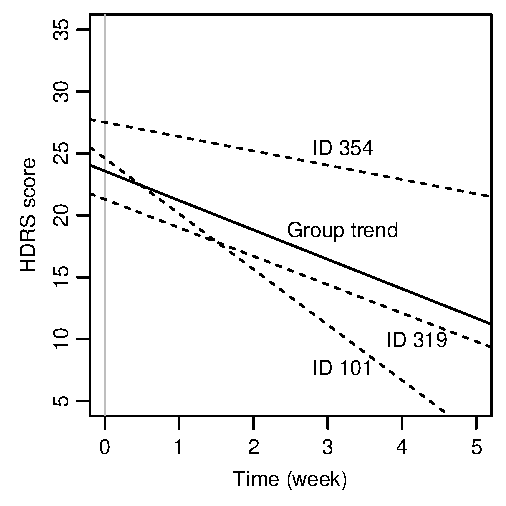
\includegraphics[width=6cm]{figures/hdrs-lme2}
\end{column}
%
\begin{column}{5cm}
  The estimated mean baseline HDRS score is $\hat{\beta}_0 = 23.58$

  The estimated standard deviation between patients is
  $\hat{\sigma}_{\upsilon_0} = 3.55$\\[2ex]

  The mean improvement per week is $\hat{\beta}_1 = -2.38$

  The estimated standard deviation between patients is
  $\hat{\sigma}_{\upsilon_1} = 1.44$\\[2ex]
\end{column}
\end{columns}
The estimated correlation between individual intercepts and slopes is
$\hat{\varrho}_{\upsilon_0 \upsilon_1} = -0.28$
  
  Patients with higher (that means worse) baseline scores improve more
  strongly than patients with smaller baseline scores
\end{frame}

\begin{frame}{Implied marginal covariance matrix}
For the three time points $t_{ij} = 0, 1, 2$,
\[
  \mat{Z}_i =
    \begin{pmatrix}
      1 & 0 \\
      1 & 1 \\
      1 & 2 \\
    \end{pmatrix}
  \text{ und }
  \gmat{\Sigma}_\upsilon =
    \begin{pmatrix}
      \sigma^2_{\upsilon_0} & \sigma_{\upsilon_0 \upsilon_1} \\
      \sigma_{\upsilon_0 \upsilon_1} & \sigma^2_{\upsilon_1}
    \end{pmatrix}
\]
we get
\begin{align*}
  & Cov(\vect{y}_i) =
    \mat{Z}_i \gmat{\Sigma}_\upsilon \mat{Z}'_i + \sigma^2 \mat{I}_{n_i} \\
  &= \begin{pmatrix}
    \sigma^2_{\upsilon_0}                                    & \sigma^2_{\upsilon_0} + \sigma_{\upsilon_0 \upsilon_1}                             & \sigma^2_{\upsilon_0} + 2 \sigma_{\upsilon_0 \upsilon_1} \\
    \sigma^2_{\upsilon_0} + \sigma_{\upsilon_0 \upsilon_1}   & \sigma^2_{\upsilon_0} + 2 \sigma_{\upsilon_0 \upsilon_1} + \sigma^2_{\upsilon_1}   & \sigma^2_{\upsilon_0} + 3 \sigma_{\upsilon_0 \upsilon_1} + 2 \sigma^2_{\upsilon_1} \\
    \sigma^2_{\upsilon_0} + 2 \sigma_{\upsilon_0 \upsilon_1} & \sigma^2_{\upsilon_0} + 3 \sigma_{\upsilon_0 \upsilon_1} + 2 \sigma^2_{\upsilon_1} & \sigma^2_{\upsilon_0} + 4 \sigma_{\upsilon_0 \upsilon_1} + 4 \sigma^2_{\upsilon_1} \\
  \end{pmatrix}
   + \sigma^2 \mat{I}_{n_i}
\end{align*}
hence, a more flexible covariance structure when compared to compound
  symmetry
\end{frame}
 
% \begin{frame}{Wald test}
% For the fixed effects, based on the covariance matrix
% \[
%   Var(\gvect{\hat\beta}) = \left( \sum_{i = 1}^N
%     \mat{X}'_i \gmat{\Sigma}_i^{-1} \mat{X}_i \right)^{-1}
% \]
% we can construct Wald tests analogously to the regular linear model with
%   approximately normally or $t$ distributed test statistics\\[2ex]
% 
%   First, $\gmat{\Sigma}_i$ must be estimated; hence, the quality of the
%   approximation strongly depends on the quality of the estimation of the
%   variance and covariance components\\[2ex]
% 
%   Many authors principally discourage using Wald tests for random effects
%   \citep[e.\,g.,][p.~52]{HedekerGibbons06}
% \end{frame}
% 
% 
% \begin{frame}{Likelihood ratio test}
%   Hypotheses about fixed and random effects can be tested with likelihood
%   ratio tests\\[2ex]
% 
%   When $M_0$ is a model that results from a more general model $M_1$ by
%   parameter restrictions, then the test statistic
% \[
%   G^2 = 2\log \frac{L(M_1)}{L(M_0)}
%       = 2\,(\log L(M_1) - \log L(M_0))
% \]
%   is approximately $\chi^2$ distributed with $(\text{Number of parameters
%   in } M_1) - (\text{Number of parameters in } M_0)$ degrees of
%   freedom\\[2ex]
% 
%   However, for fixed effects this test can result in progressive test
%   decisions for small samples (H$_0$ is rejected too often)\\[2ex]
%   
%   For random effects and hypotheses of the form H$_0$: $\sigma^2_\upsilon =
%   0$, the test is rather conservative
%   \nocite{BrykRaudenbush2002}
% \end{frame}



% \begin{frame}{Mixed-effects models}
%   \begin{itemize}
%     \item Mixed-effects models are a class of statistical models that
%       include fixed effects as well as random effects
%     \item Fixed effects vs.\ random effects\footnote{Some critical
%       discussion on these definitions:
%       \url{http://andrewgelman.com/2005/01/25/why_i_dont_use/}}
%     \begin{itemize}
%       \item For fixed effects, only effects of the factor levels used in the
%         present study are considered (manipulated levels, e.\,g., groups,
%         sex, \dots)\\[1ex]
% 
%         $\to$ Of interest is how these levels differ
%       \item For random effects, the factor levels considered in a study are
%         regarded as a (random) sample from some population (e.\,g., words,
%         raters, subjects, \dots)\\[1ex]
% 
%         $\to$ Of interest are conlusions about the underlying population and its
%         variation
%     \end{itemize}
%   \end{itemize}
% \end{frame}

% \begin{frame}{Data schema for dependent data}
%   \small
% \begin{columns}
%   \column{.65\textwidth}
% \begin{tabular}{cccccc}
% \hline
% Person & Time      & Observ.     & \multicolumn{3}{c}{Covariates}\\\hline
% 1      & 1         & $y_{11}$    & $x_{111}$   & \dots & $x_{11p}$  \\
% 1      & 2         & $y_{12}$    & $x_{121}$   & \dots & $x_{12p}$  \\
% .      & .         & .           & .           & \dots & .          \\
% 1      & $n_1$     & $y_{1n_1}$  & $x_{1n_11}$ & \dots & $x_{1n_1p}$\\
% .      & .         & .           & .           & \dots & .          \\
% .      & .         & .           & .           & \dots & .          \\
% $N$    & 1         & $y_{N1}$    & $x_{N11}$   & \dots & $x_{N1p}$  \\
% $N$    & 2         & $y_{N2}$    & $x_{N21}$   & \dots & $x_{N2p}$  \\
% .      & .         & .           & .           & \dots & .          \\
% $N$    & $n_N$     & $y_{Nn_N}$  & $x_{Nn_N1}$ & \dots & $x_{Nn_Np}$\\
% \hline
% \end{tabular}
% %
%   \column{.45\textwidth}
% \begin{itemize}
% \item $i = 1, \dots, N$ persons
% \item $j = 1, \dots, n_i$ time points for person $i$
% \item All observations: $\sum_i^N n_i$
% \item Vector of all observations for person $i$\\
%   $(\vect{y}_i)_{n_i \times 1}$\\
% \item Vector of covariates for person $i$ at time point $j$\\
%   $(\vect{x}_{ij})_{p \times 1}$
% \item All covariates of person $i$\\
%   $(\vect{X}_i)_{n_i \times p}$
% \end{itemize}
% \end{columns}
% \end{frame}

\begin{frame}{Linear mixed-effects model}
  \begin{itemize}
    \item The linear mixed-effects model has the general form
\[
  \vect{y}_i = \mat{X}_i \, \gvect{\beta} + \mat{Z}_i \, \gvect{\upsilon}_i +
               \gvect{\varepsilon}_i
\]
with fixed effects $\gvect{\beta}$, random effects
$\gvect{\upsilon}_i$, and the design matrices $\mat{X}_i$ and $\mat{Z}_i$
  and the assumptions
\[
  \gvect{\upsilon}_i \sim N(\vect{0}, \, \gmat{\Sigma}_\upsilon)
    \text{ i.i.d.}, \qquad
  \gvect{\varepsilon}_i \sim N(\vect{0}, \, \sigma^2 \mat{I}_{n_i})
    \text{ i.i.d.}
\]
\item This implies for the marginal covariance matrix
\[
  Cov(\vect{y}_i) = \gmat{\Sigma}_i =
    \mat{Z}_i \gmat{\Sigma}_\upsilon \mat{Z}'_i + \sigma^2 \mat{I}_{n_i}
\]
%\item The linear mixed-effects model has many special cases including
%  hierarchical and multilevel models as well as models for longitudinal
%  data
  \end{itemize}
\end{frame}

\begin{frame}[shrink=25]{Linear mixed-effects model}
\vspace{2cm}
\begin{equation*}
  \begin{pmatrix}
    y_1 \\
    y_2 \\
    y_3 \\
    \vdots \\
    y_N
  \end{pmatrix} = 
  \begin{pmatrix}
    1 & x_{11} & x_{12} & \dots & x_{1p} \\
    1 & x_{21} & x_{22} & \dots & x_{2p} \\
    1 & x_{31} & x_{32} & \dots & x_{3p} \\
    \vdots & \vdots & \vdots & \vdots & \vdots \\
    1 & x_{N1} & x_{N2} & \dots & x_{Np} \\
  \end{pmatrix} \cdot
  \begin{pmatrix}
    \beta_0 \\
    \beta_1 \\
    \vdots \\
    \beta_p
  \end{pmatrix} +
  \begin{pmatrix}
    z_{10} & z_{11} & \dots & z_{1q} & \dots \\
    z_{20} & z_{21} & \dots & z_{2q} & \dots \\
    z_{30} & z_{31} & \dots & z_{3q} & \dots \\
    \vdots & \vdots & \vdots & \vdots & \vdots \\
    z_{N0} & z_{N1} & \dots & z_{Nq} & \dots \\
  \end{pmatrix} \cdot
  \begin{pmatrix}
    \upsilon_{10} \\
    \vdots \\
    \upsilon_{1q}\\
    \upsilon_{20} \\
    \vdots \\
    \upsilon_{Nq}
  \end{pmatrix} + 
  \begin{pmatrix}
    \varepsilon_1 \\
    \varepsilon_2 \\
    \varepsilon_3 \\
    \vdots \\
    \varepsilon_N
  \end{pmatrix}
\end{equation*}
\end{frame}

% \begin{frame}[fragile]{Structure of data}
%   \begin{lstlisting}
% > xtabs( ~ Subject + Days, sleepstudy)
%        Days
% Subject 0 1 2 3 4 5 6 7 8 9
%     308 1 1 1 1 1 1 1 1 1 1
%     309 1 1 1 1 1 1 1 1 1 1
%     310 1 1 1 1 1 1 1 1 1 1
%     330 1 1 1 1 1 1 1 1 1 1
%     331 1 1 1 1 1 1 1 1 1 1
%     332 1 1 1 1 1 1 1 1 1 1
%     333 1 1 1 1 1 1 1 1 1 1
%     334 1 1 1 1 1 1 1 1 1 1
%     335 1 1 1 1 1 1 1 1 1 1
%     337 1 1 1 1 1 1 1 1 1 1
%     349 1 1 1 1 1 1 1 1 1 1
%     350 1 1 1 1 1 1 1 1 1 1
%     351 1 1 1 1 1 1 1 1 1 1
%     ...
%   \end{lstlisting}
% \end{frame}

% {\setbeamercolor{background canvas}{bg=iwmgrau!80!white}
% 
% \begin{frame}[fragile]{}
%   \begin{lstlisting}
%   ##
%   \end{lstlisting}
% \end{frame}
% 
% }
% 
% \begin{frame}[fragile]{}
%   \begin{block}{Exercise}
%     \begin{itemize}
%       \item 
%     \end{itemize}
%   \end{block}
% \end{frame}

\appendix
%\begin{frame}[allowframebreaks]{References}
\begin{frame}{References}
%\renewcommand{\bibfont}{\footnotesize}
\bibliographystyle{apacite}
\bibliography{../../../literature/nu}
\vfill
\end{frame}

\end{document}

